\documentclass[]{final_report}
\usepackage{graphicx}
\usepackage{hyperref}
\usepackage{longtable}
\usepackage{wrapfig}
\usepackage{mathtools}


%%%%%%%%%%%%%%%%%%%%%%
%%% Input project details
\def\studentname{Eman Naveed}
\def\reportyear{2024}
\def\projecttitle{Lindenmayer Systems}
\def\supervisorname{Anand Subramoney}
\def\degree{MSci (Hons) in Computer Science}
\def\fullOrHalfUnit{Full Unit} % indicate if you are doing the project as a Full Unit or Half Unit
\def\finalOrInterim{Final Report} % indicate if this document is your Final Report or Interim Report

\begin{document}

\maketitle

%%%%%%%%%%%%%%%%%%%%%%
%%% Declaration
\chapter*{Declaration}

This report has been prepared on the basis of my own work. Where other published and unpublished source materials have been used, these have been acknowledged.

\vskip3em

Word Count: 

\vskip3em

Student Name: \studentname

\vskip3em

Date of Submission: 

\vskip3em

Signature: Eman Naveed

\newpage

%%%%%%%%%%%%%%%%%%%%%%
%%% Table of Contents
\tableofcontents\pdfbookmark[0]{Table of Contents}{toc}\newpage

%%%%%%%%%%%%%%%%%%%%%%
%%% Your Abstract here

\begin{abstract}

Lindenmayer Systems, since their introduction, have been used extensively to model natural structures. From simple computer graphics to advanced medical research, this method of rewriting strings and translating them into graphical output has been vital in producing accurate mimics of organic structures. 

Although first proposed as a theory to help study plant growth, it is easy to find uses of them in various other fields. In medicine, they have been used to create models of the human genome and replicate arterial branching of the cardiovascular system. There is mention of them in paleobiological research, aiding virtual recreation of fossils from broken remains to allow further study of extinct organisms. There is use of them in music even, producing complex scores with still legible internal structure, the results as attractive in musical applications as in graphics.

This project aims to explore the different classes of L-systems and provide an implementation in Java that allows the user to see the differences in productions when using these different classes. 


\end{abstract}

%%%%%%%%%%%%%%%%%%%%%%
%%% Introduction
\chapter{Introduction}

Lindenmayer systems (L-systems)~\cite{PRU:1990} are parallel rewriting systems based on formal grammars. They consist of character strings and a set of production rules to define rewriting, and | due to their initial use as modelling aids | a method of translating these characters into some form of graphical output.

This system was introduced and developed in 1968 by Aristid Lindenmayer, a biologist and botanist, and presented a way to model plant growth and study the replicating behaviour of plant cells. There are several different kinds of l-systems with their specific functionalities and outputs differing according to the rules they follow. Since their introduction, there have been many methods used to convert the productions created from these systems into graphical output to aid understanding of plant morphology~\cite{CUR:1999}~\cite{BUR:2013}~\cite{HEW:2017}~\cite{CGO:1997}. The method explored in this project, makes use of Java and Processing 4.3 for the background code and graphical output.

\section{Problem Statement}

The objective of this project was to research and report on the different types of l-systems and how those differences relate to their purpose, and implement simple fractals and stochastic productions, connecting the outputs and their methods of creation to the mimicking of plant growth and evolution. Another objective was to develop a working GUI-based l-system environment that demonstrated skills with Java and related graphics frameworks.

\section{Outline}

This report provides background theory on the functionality of l-systems. It explores the various classes of l-systems and how the differences between those classes affects how they are utilized in research and computation. An overview is also given on the method of visualization of output. Chapter 3 then explains the approach taken with  coding, discussing initial steps, how the program is divide, and the alterations made to the initial design in extending functionality to get to the final product. A section on professional issues discusses some problems that concern this project. Some possible future extensions are explored within the conclusion.

\section{Motivation}

L-systems are used extensively to research plant growth in more ways than just looking at cell reproduction and replication. These systems have been modified to consider interactions between objects as well, taking into account geographical distribution, population genetics, epidemics and more factors to help researchers understand environmental development and create accurate simulations where necessary.~\cite{DGG:1997} 

What proved intriguing to me during my initial research was the way in which these kinds of systems have been utilized in other fields of research. In medicine, they have been used to focus on arterial branching~\cite{ZAM:2001} and the human gene~\cite{GOS:2010}; there is use of them in the context of music, creating playable melodies.

\begin{wrapfigure}{r}{0.45\textwidth}
\centering
\begin{minipage}[c]{6.5cm}
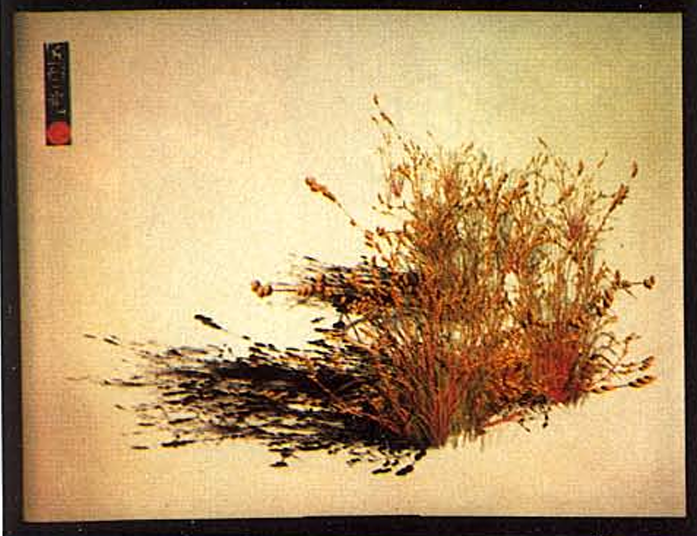
\includegraphics[width=6.5cm]{whiteSands.png} 
\caption{\label{fig:AlvyRay} Several 3D renderings of a context-sensitive grammar mixed with particle system grasses. Source:~\cite{ARS:1984}}
\end{minipage}
\end{wrapfigure}
Their implementation in creating art is also its own marvel. An architect, Michael Hansmeyer~\cite{HAN:2003}, has a page on his website dedicated to 3D productions obtained through various kinds of l-systems. Alvy Ray Smith, the co-founder of Pixar, explored the use of l-systems in efficiently generating landscapes. In his paper~\cite{ARS:1984}, he makes note of the way in which they can be used in conjunction with other rendering systems and painting methods to obtain complex images with the use of only a small database. While I have no evidence that l-systems are actually used in animation today, the thought of it was interesting enough to make me curious to know more.

Before project selection began, I also found a research paper that used l-systems to reconstruct a fossil. The paper explained how using parametric l-systems to create reconstructions of these organisms revealed a fractal, self-similar nature to their structures that explained how they maximized surface area. The discovery stood consistent with what was know about their uptake of nutrients in water columns, and the resulting 3D reconstruction closely matched the anatomy of the fossil specimen.~\cite{HOY:2014}

There was enough use of these systems across such vast and seemingly unrelated fields that I saw this being something that would prove useful to me as a personal project as well. It overlapped with so many fields that I had considered in passing and had wanted better understanding of. I saw this project as something I could continue developing even after the official submission of it in university context; something that would hold my attention and allow me to explore implementation of graphics and their varied applications. The research papers I found related to l-systems in particular | and even those focused on fractal geometry | opened my mind to possibilities of using l-systems in making designs for fabric crafts that I have an interest in. I wanted to work on 3D l-systems, though I did not manage that much during the duration of this project; I wanted to explore the kind of objects that could be built from it. The fossil reconstruction was a particular interest that grabbed my attention and I hope to develop the end product into something that has 3D capability  and can create shell structures such as those of ammonite fossils, and perhaps progress into realistic landscapes with a mix of graphics systems as described by Smith~\cite{ARS:1984}.

\chapter{Background Theory}

L-systems were introduced as a method of simulating multicellular organisms, but have since been utilized in varied fields outside of biology and computing as well. These systems were originally conceived as linear arrays of interconnected finite automata, each automaton corresponding to a living cell, with the possibility that new automata can be added to the array (cells divide) or be deleted from the array (cells die)~\cite{LIN:1972}. 

L-systems now make use of a starting character string, an \emph{axiom}, and consist of a rule or series of rules, the \emph{generators} or \emph{production rules}. At each point in the generation, every character that has a production rule corresponding to it is rewritten simultaneously and the changes are carried out on the resulting figure as a whole. As we generate more productions using these rules, the size of the string output increases exponentially as well as the complexity of the resulting structure produced.

The rewriting of l-systems differs from traditional grammars in its parallel execution, as most traditional grammars execute sequentially. So, for example~\cite{ROZ:1974}, if a character \textit{S} is to be replaced with the string \textit{SS} and you are starting with the axiom \textit{S}, the resulting string, both with sequential rewriting and parallel, would be \textit{SS}. But in the next generation, traditional grammars would give us the string \textit{SSS}, while l-system rewriting would give us \textit{SSSS} as all characters would be rewritten at once. While most self-similar structures can be replicated easier with l-systems because of this property, in instances where the first outcome(\textit{SSS}) is required, they would not be feasible.

\begin{figure}[h]
\centering
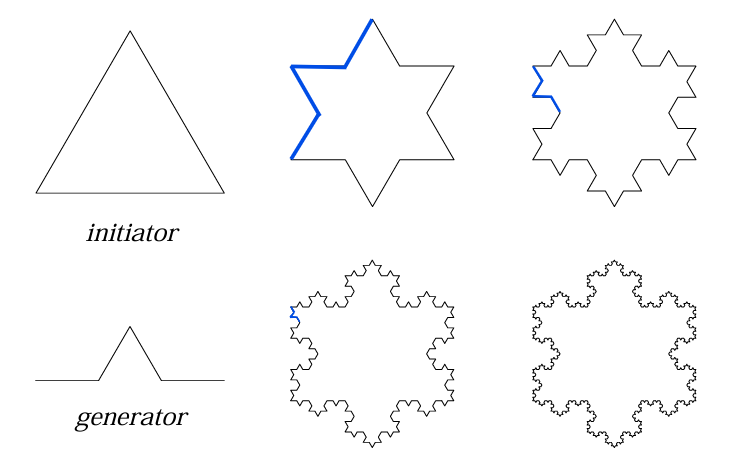
\includegraphics[width=12cm]{koch_curve} 
\caption{\label{fig:koch_curve} Construction of the Koch snowflake curve.}
\end{figure}

The above figure demonstrates the concept of parallel rewriting visually using the Koch snowflake as an example. The $initiator$ takes place of the axiom, and the $generator$ presents as the production rule for every straight line. While the generator replaces all straight lines in each production, the shape as a whole remains geometrically similar, demonstrating the self-similarity of the fractal and the generator that creates it~\cite{MAN:1982}.

\section{Turtle Visualization}

The basic visual depictions of l-systems could be expressed using any simple graphics but in order to model higher plants, more sophisticated graphical interpretations were required. The first results towards this goal were published by Frijters and Lindenmayer~\cite{FRJ:1974}, and Hogeweg and Hesper~\cite{HOG:1974}. Both methods used l-systems to sort out branching topology with the geometrical aspects such as the length of line segments and angle values added in a post-processing phase. The Hogeweg and Hesper interpretations were used by Smith~\cite{ARS:1984} to showcase truly realistic graphics.

Szilard and Quinton observed that L-systems could be applied to generate a variety of intricate geometric patterns if graphical interpretation was associated with specific symbols in the generated strings~\cite{ZIL:1979}. They made use of a technique in which strings defined images according to the chain coding mechanism~\cite{FRE:1961}. There were multiple simulation programs such as CELIA~\cite{CEL:1970} that were either based on or made for l-systems. Prusinkiewicz then proposed the use of a more LOGO-style turtle interpretation~\cite{TRT:1981}. This presented a way to develop fractals and plant-like images with simple graphics~\cite{PRU:1996}, but was also extended by many others in various directions to simulate realistic high-complexity models.

Turtle interpretation has a \emph{state} defined for the \emph{turtle} as a triplet $(x, y, \alpha)$, where the Cartesian coordinates $(x, y)$ represents the \emph{position} of the \emph{turtle}, and the angle $\alpha$ is interpreted as the direction in which the \emph{turtle} is facing. Given a \emph{step size d} and the \emph{angle increment $\delta$}, the turtle can respond to commands represented by the following symbols:

\begin{center}
\begin{minipage}[c]{0.75\linewidth}
    \begin{description}
        \item[F] Move forward a step of length $d$. The state of turtle is updated to $(x', y', \alpha)$ and a line segment is drawn between points $(x, y)$ and $(x', y')$.
        \item[$+$] Turn left by angle $\delta$. The new state of the turtle is $(x, y, \alpha + \delta)$. The positive orientation of angles is counter-clockwise.
        \item[$-$] Turn right by angle $\delta$. The new state of the turtle is $(x, y, \alpha - \delta)$.
    \end{description}
\end{minipage}
\end{center}

Given a string $v$, the initial state of a turtle $(x_0 , y_0, \alpha_0)$ and fixed parameters $d$ and $\delta$, the \emph{turtle interpretation} of $v$ is the figure (set of lines) drawn that corresponds to the string $v$ | as shown in the following figure.

\begin{figure}[h]
    \begin{minipage}[c]{0.5\linewidth}
        \centering
        (a)
        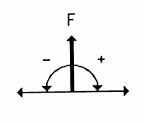
\includegraphics[width=4.5cm]{turtle.png}
    \end{minipage}\hfill
    \begin{minipage}[c]{0.5\linewidth}
        \centering
        (b)
        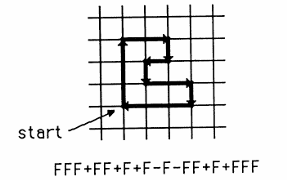
\includegraphics{turtlegrid.png}
    \end{minipage}
    \caption{\centering(a) Turtle interpretation of string symbols F, +, -. (b)Interpretation of a string. The angle increment $\theta$ is equal to $90^{\circ}$. The turtle faces up initially. Source:~\cite{HAN:1989}.}
\end{figure}

This method can be applied to interpret strings generated by l-systems, and is the one used in this project. Another example of the fractals that can be generated from this method is given below. The images generated stem from derivations 1 to 4 of a quadratic variation of the Koch snowflake shown in Figure \ref{fig:koch_curve}. The axiom and rule for these productions are as follows:

\begin{center}
\begin{minipage}[c]{0.25\linewidth}
    \begin{description}
        \item[$\omega$] $\rightarrow$ -F
        \item[F] $\rightarrow$ F-F+F+F-F
    \end{description}
\end{minipage}
\end{center}

\begin{figure}
    \centering
    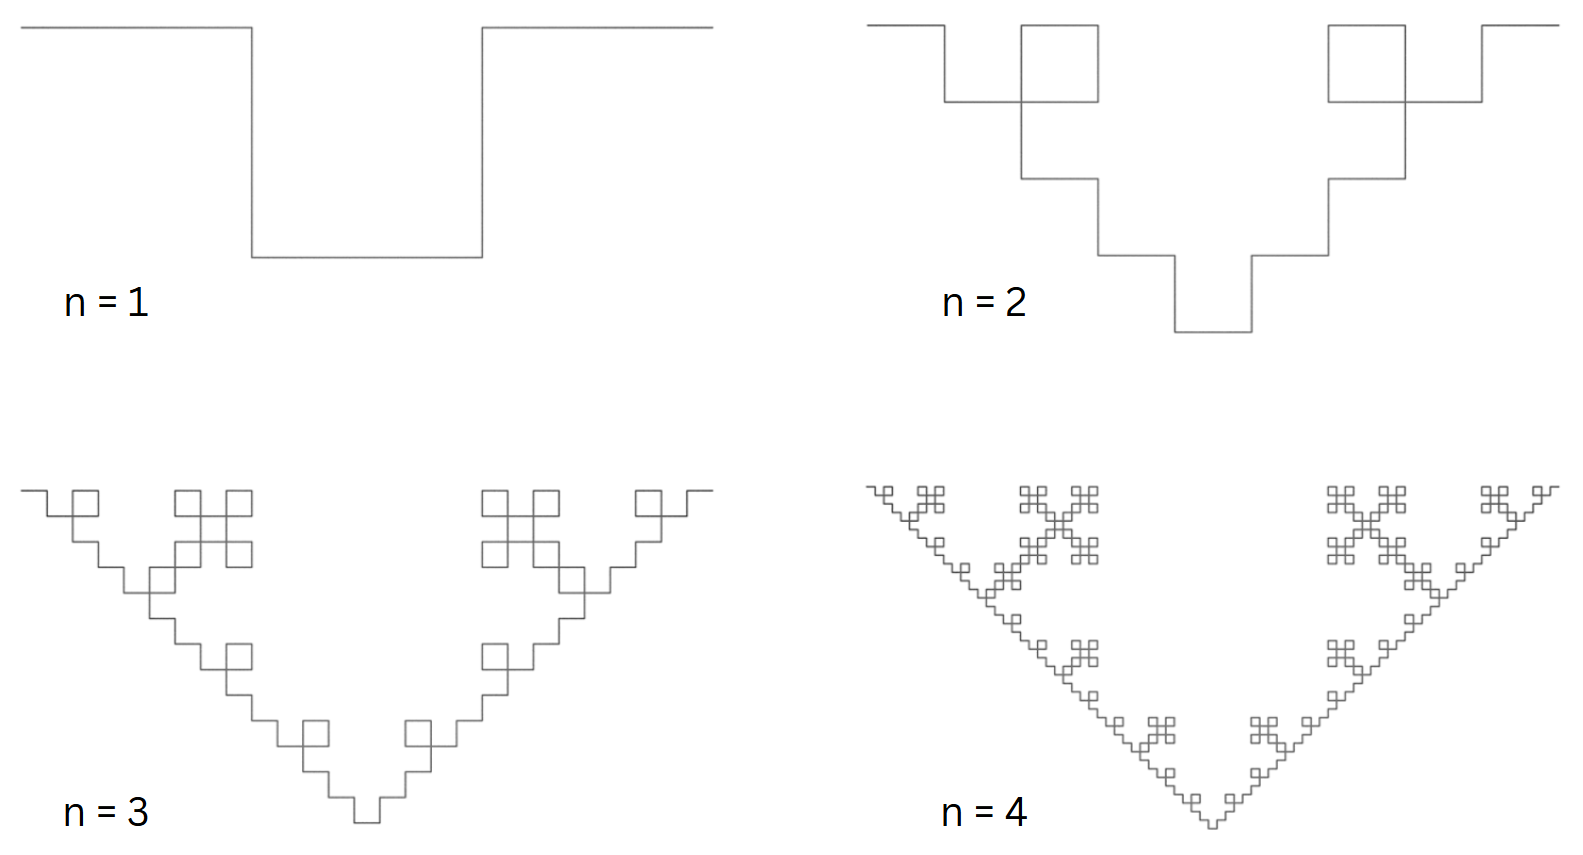
\includegraphics[width=12cm]{quadKoch.png}
    \caption{Generating a quadratic modification of the Koch snowflake.}
    \label{fig:quadraticKoch}
\end{figure}

\section{Classes of L-Systems}

It is important to understand the concept behind the different kinds of L-systems and how these distinctions affect the output. L-systems can broadly be classified using two axes: (1) deterministic or stochastic, and (2) context-free or context-sensitive~\cite{NANA:2010}. In the following subsections, context-free versions of deterministic (D0L) and stochastic (S0L) systems will be discussed separately and context-sensitive (IL) systems will be discussed collectively. The section on parametric l-systems explain a class that is unrelated to the ones mentioned previously, but stands just as important outside the main classifications.

\subsection*{D0L-Systems}

The simplest class of L-systems are called D0L-systems (deterministic context-free L-systems). This is the kind of L-system that results in the commonly seen self-similar fractals. In the context of this class of L-system, there are individual rules corresponding to a character, so a system is deterministic if and only if for each letter that is part of the specified alphabet, there is exactly one or no generator related to it. To understand better, we can explore an example. 
\begin{figure}[h]
    \centering
	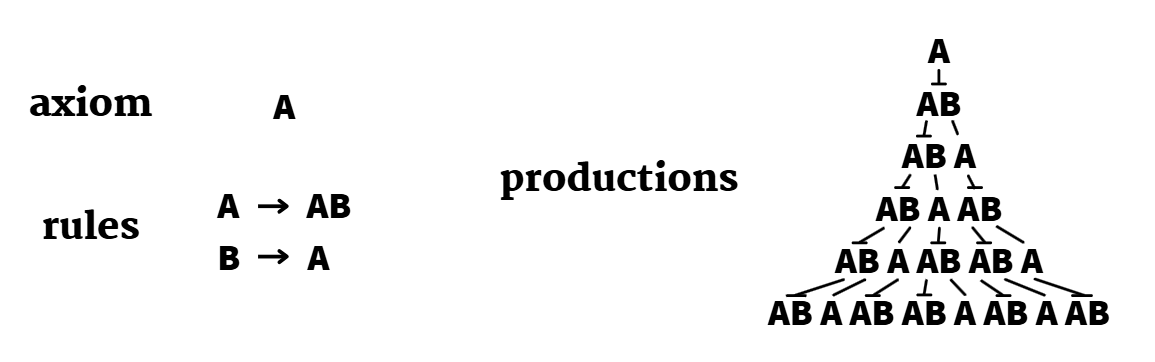
\includegraphics[width=12cm]{axRuleProd.png} 
    \caption{\label{fig:image} Example of a derivation in a D0L-system.}
\end{figure}

Consider strings built of two letters, $A$ and $B$. For each letter we specify a rewriting rule. In this case, $A \rightarrow AB$, and $B \rightarrow A$. This means that at each generation, every occurrence of $A$ will be rewritten with $AB$ and every occurrence of $B$ will be rewritten with $A$. We see this rewriting occur simultaneously across all $A$ and $B$ in each string production. Image generation with this class of L-system is also demonstrated in the introduction in Figure \ref{fig:koch_curve}. 

There have been countless extensions of the basic D0L-system model to create more complex fractals. We can see this with an approximation of the "quadratic Koch Island", beginning with the axiom $F+F+F+F$, and the production rule $F \rightarrow F+F-F-FF+F+F-F$. 

\begin{figure}[h]
    \centering
	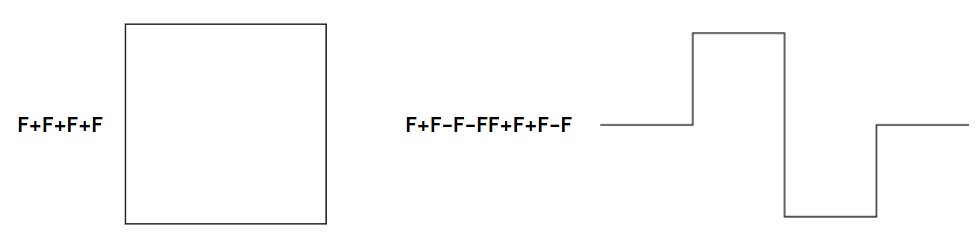
\includegraphics[width=13cm]{kochRule.png} 
    \caption{\label{fig:kochRule} Koch Island axiom and rule.}
\end{figure}

The following images correspond to the strings obtained in derivations of length 1-3, with the first image of Figure \ref{fig:kochRule} being the image for derivation of length 0.

\begin{figure}[h]
    \centering
	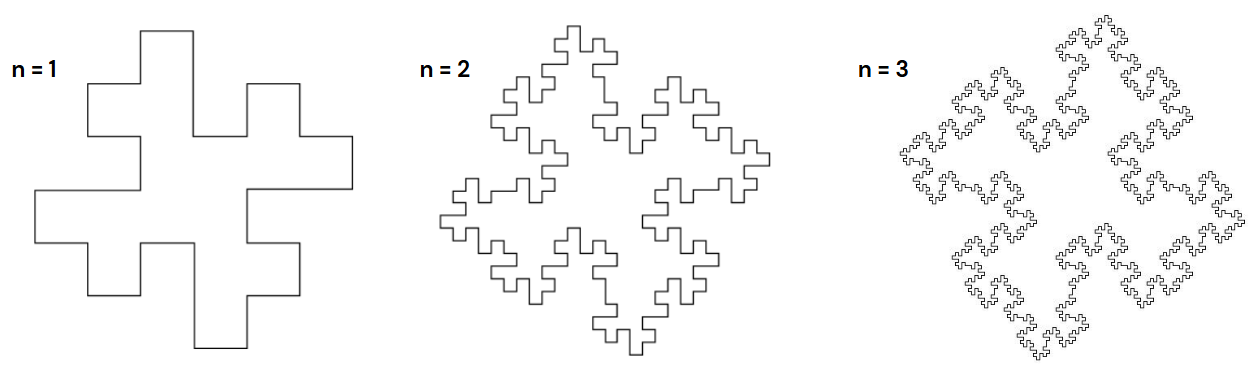
\includegraphics[width=13cm]{kochIsle.png} 
    \caption{\label{fig:image} Koch Island generations 1-3. Source:~\cite{PRU:1990}}
\end{figure} 

The angle increment $\theta$ for this structure is $90^{\circ}$. The length of the straight line drawn is decreased with each generated image. This makes the distance between the endpoints of the polygon represented by the production successor equal to the length of the line represented by the predecessor.

While fractal structures are customary with D0L-systems, their singular rewriting measures can still produce branching structures that mimic plant images to quite a high degree of 
\begin{wrapfigure}{r}{0.45\textwidth}
\centering
\begin{minipage}[c]{6.5cm}
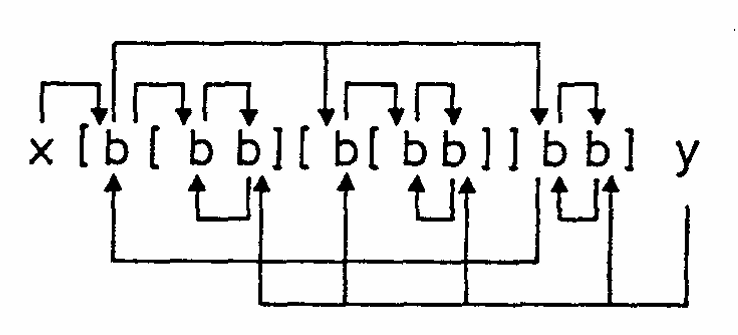
\includegraphics[width=6.5cm]{hogeweg.png} 
\caption{\label{fig:hogeweg} An example of a bracketed string. Source:~\cite{HOG:1974}}
\end{minipage}
\end{wrapfigure}accuracy. With turtle interpretation this is done with the use of brackets | \verb|[| and \verb|]|. The \verb|[| pushes the current state of the system onto a pushdown stack. All values concerning the turtle's position and orientation as well as any other parameters necessary are stored.  The \verb|]| then returns the system back to the saved position. No line is drawn in returning the turtle to the initial position. Hogeweg and Hesper describe this as the substring within the brackets being "lifted out of the string". These kinds of modular branching structures are also referred to in some areas as \emph{bracketed l-systems}. The figure below shows an example of an image produced for a bracketed l-system that I produced.

\begin{figure}[h]
    \centering
	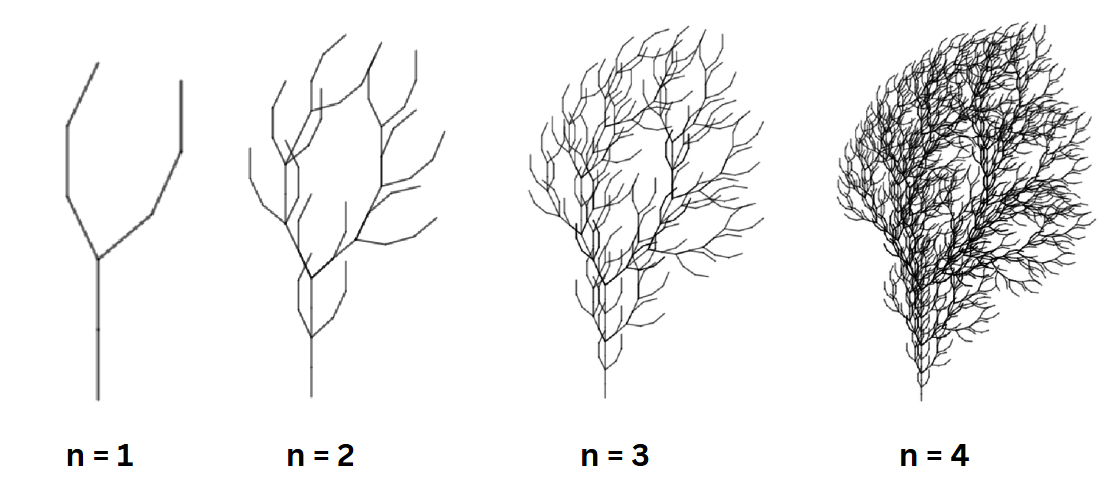
\includegraphics[width=14cm]{D0Lplant.png} 
    \caption{\label{fig:D0L} Fractal tree using D0L-system with $\theta$ = $25^{\circ}$} Axiom: F, Rule $F \rightarrow FF-[-F+F+F]+[+F-F-F]$
\end{figure}

% ADD ANOTHER D0L TREE EXAMPLE IF THERE IS TIME

\subsection*{Stochastic L-Systems}

Stochastic L-systems (S0L-systems | stochastic context-free L-systems) have the same main components of L-systems. The distinction from D0L-systems lies in the production rules and the way they are used. Stochastic L-systems integrate an extent of randomness into the produced models. Consequently, different graphical outputs can be obtained in simulations even if the initial conditions are identical for each run. The amount and direction of variation in the results depends on the chosen probability distribution that imposes structure on the simulation algorithms.

We can explore a simple example with the following rules:
\begin{figure}[h]
\begin{minipage}[c]{0.25\linewidth}
    \flushleft
    $\omega : F$\newline
    $p_1 : F \xrightarrow{.33} F[+F]F[-F]F$\newline
    $p_2 : F \xrightarrow{.33} F[+F]F$\newline
    $p_3 : F \xrightarrow{.34} F[-F]F$
\end{minipage}\hfill
\begin{minipage}[c]{0.75\linewidth}
	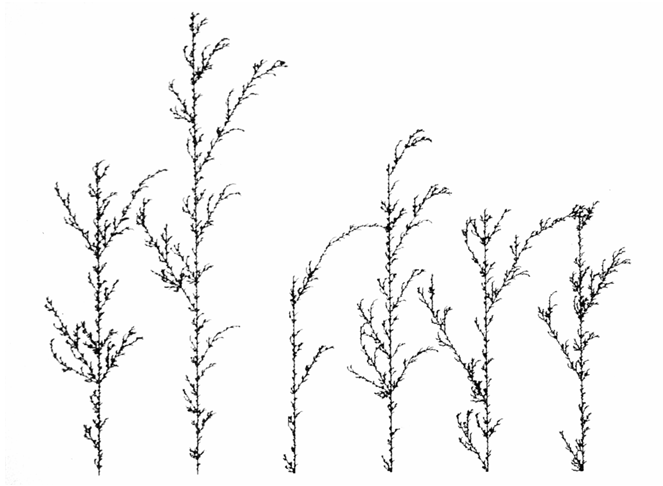
\includegraphics[width=13cm]{Stochplant.png} 
\end{minipage}
    \caption{\label{fig:sixStoch} Stochastic branching productions. Source:~\cite{PRU:1990}.}
\end{figure}

The production probability of each outcome is mentioned above the derivation symbol $\rightarrow$. Each production has a roughly 1/3 chance of being selected for the rewriting at every point of generation. Each tree in Figure \ref{fig:sixStoch} begins with the same axiom and uses the same set of rules. All lines drawn are of the same unit length and use the same angle of rotation at branching points, yet we can see numerous differences in each of the final products. The same factors hold for the tree images in Figure \ref{fig:myStoch}.

\begin{figure}[h]
    \centering
	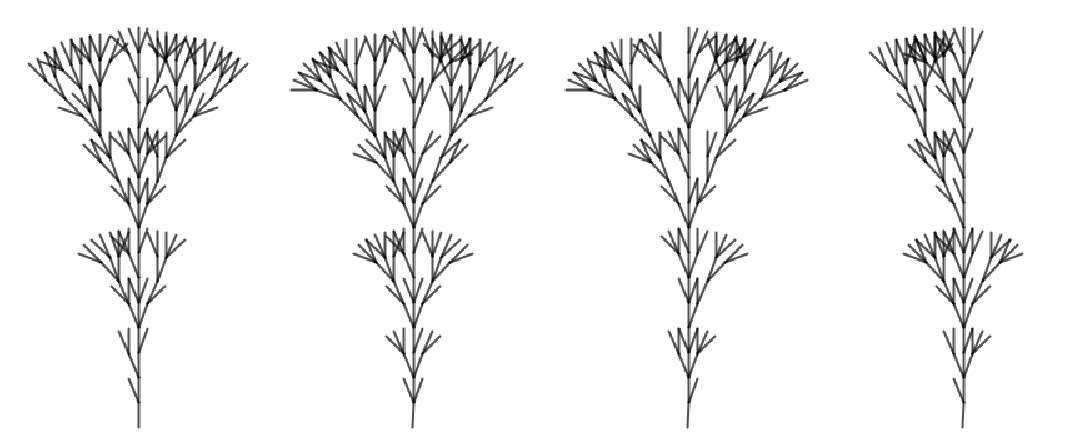
\includegraphics[width=14cm]{Stoch2.png} 
    \begin{center}
        \begin{minipage}[c]{5cm}
            %$\omega : F$, $\theta : 22.5^{\circ}$\newline
            $p_1 : F \xrightarrow{.50} F[+F][-F]F$\newline
            $p_2 : F \xrightarrow{.30} F[-F]F$\newline
            $p_3 : F \xrightarrow{.20} F[+F]F$
        \end{minipage}
    \end{center}
    \caption{\label{fig:myStoch} Four objects produced using stochastic L-systems.}
\end{figure}

S0L-systems provide the opportunity to create different classes of plants, all sharing overall similar characteristics but differing in minor details. The rules used for the images in Figures \ref{fig:sixStoch} and \ref{fig:myStoch} are not dissimilar, yet the productions are completely different and would not fit in the same fictitious class of plants. While these examples are fairly simple in nature, they already look quite plant-like. There has been implementation that directly attempted to mimic specific plant species by creating a complex table of rules using an extensive alphabet for tiny sections of a singular leaf~\cite{KOL:1980} with the results coming quite close to the observed specimen.

There is research on the reverse engineering of these systems as well, using them to potentially identify plants instead of simulate them. The experiment saw the researchers generating plants using stochastic l-systems which were then used for the training and test sets. The final model, had a very high accuracy for identification by shape and identification by branch structure despite the initial hypothesis that it would not be too successful due to the random probabilistic nature of the generations. It resulted in the authors considering the use of similar l-system based models to recognize natural plants by shape.~\cite{ASH:1994}

\subsection*{Context-Sensitive L-Systems}

Productions of context-free systems remain consistent regardless of a previous state, however, there is functionality to change the behaviour of systems according to the state of a neighbour or predecessor. Context-sensitive l-systems allow researchers to simulate and study factors such as nutrient flow and hormones by considering the state of neighbours and generating the next production accordingly.

Generally \emph{2L-systems} have the format $a_l < a > a_r \rightarrow \chi$, where the letter $a$ | considered the \emph{strict predecessor} | can produce a sentence $\chi$ if and only if $a$ is preceded by a letter $a_l$ and followed by a letter $a_r$~\cite{HAN:1989}. In this way, the letters $a_l$ and $a_r$ provide the left and right \emph{context} of $a$ in this production. Productions in \emph{1L-systems} carry one-sided context only, so they either exist in the form $a_l < a \rightarrow \chi$ or $a > a_r \rightarrow \chi$. \emph{0L-systems}, \emph{1L-systems}, and \emph{2L-systems} all belong to a wider class of \emph{IL-systems}, also called $<k,l>$\emph{L-systems}. In a $<k,l>$L-system, the left context is a word of length $k$, whereas the right context is word of length $l$. Lindenmayer and Rozenberg refer to these inputs as \emph{neighbourhoods} and explain that the biological interpretation of said \emph{neighbourhoods} has to do with the transport of substances from cell to cell, and with their activity as inducers or inhibitors of enzymes~\cite{LIN:1972}.

In an effort to keep l-system descriptions short, most papers modify the usual notion of IL-systems to allow allow productions of different context lengths to coexist within a single system. Because of this, if a context-free and a context-sensitive production exist together in a system and apply to the same letter, the context-sensitive production would be selected for rewriting.

\begin{figure}[h]
\centering
        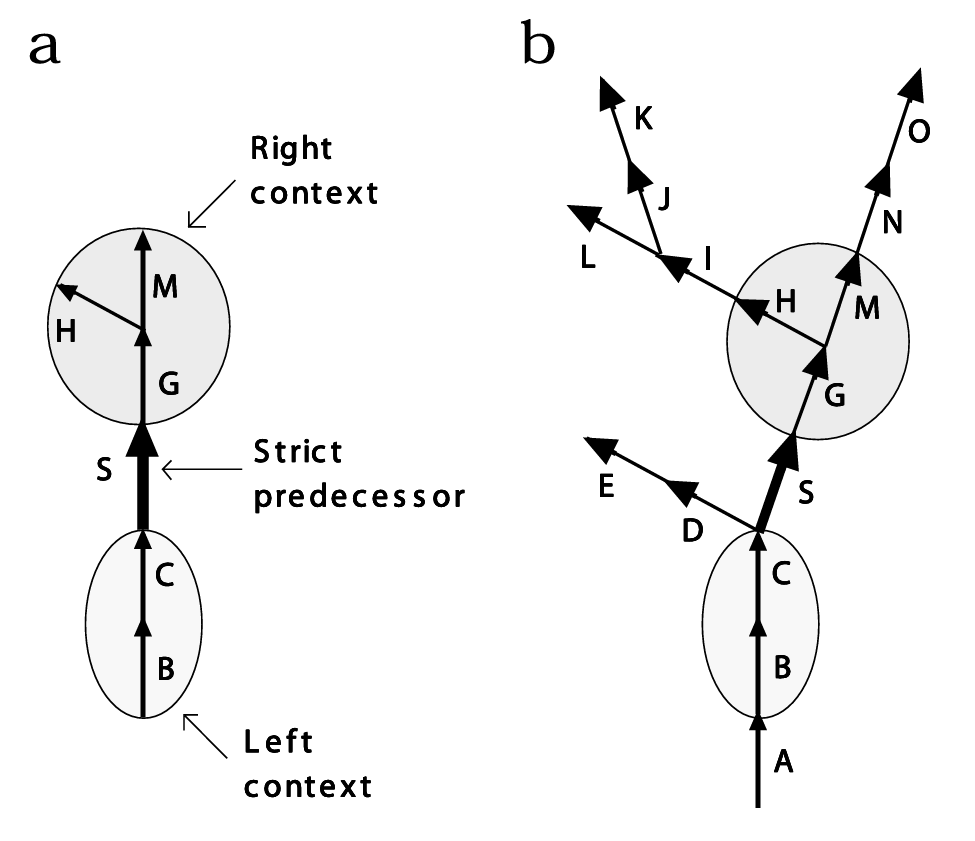
\includegraphics[width=10cm]{strictPred.png}
    \begin{minipage}[c]{12cm}
        \caption{\centering The predecessor of a context-sensitive tree production (a) matches edge S in a tree T (b). Source:~\cite{PRU:1996}}
        \label{fig:strict}
    \end{minipage}
\end{figure}

We can use a simple example to simulate signal propagation through a string of characters:
\begin{center}
    \begin{minipage}[c]{2.5cm}
        $\omega:$ \textit{baaaaaaa}\newline
        $p_1$: $b>a \rightarrow b$\newline
        $p_2$: $b \rightarrow a$
    \end{minipage}
\end{center}
These rules have the character $b$ moving across the string from the left to the right. The first few words generated by this are given below:
\begin{center}
    \begin{minipage}[c]{2cm}
        \textit{baaaaaaa}\newline
        \textit{abaaaaaa}\newline
        \textit{aabaaaaa}\newline
        \textit{aaabaaaa}\newline
        ...
    \end{minipage}
\end{center}
The use of context in bracketed systems is a bit more complex than with 0L-systems. With bracketed systems, characters representing tree segments can be separated by an arbitrarily large number of characters in between~\cite{HAN:1989}. For example, Figure \ref{fig:strict} indicates that a a production with the predecessor $BC<S>G[H]M$ can be applied to character $S$ in the string
\begin{center}
    \begin{minipage}[c]{5cm}
        $ABC[DE][SG[HI[JK]L]MNO]$,
    \end{minipage}
\end{center}
which involves skipping over characters $[DE]$ while searching for left context and $I[JK]L$ while searching for right context. 

\begin{figure}[h]
    \centering
    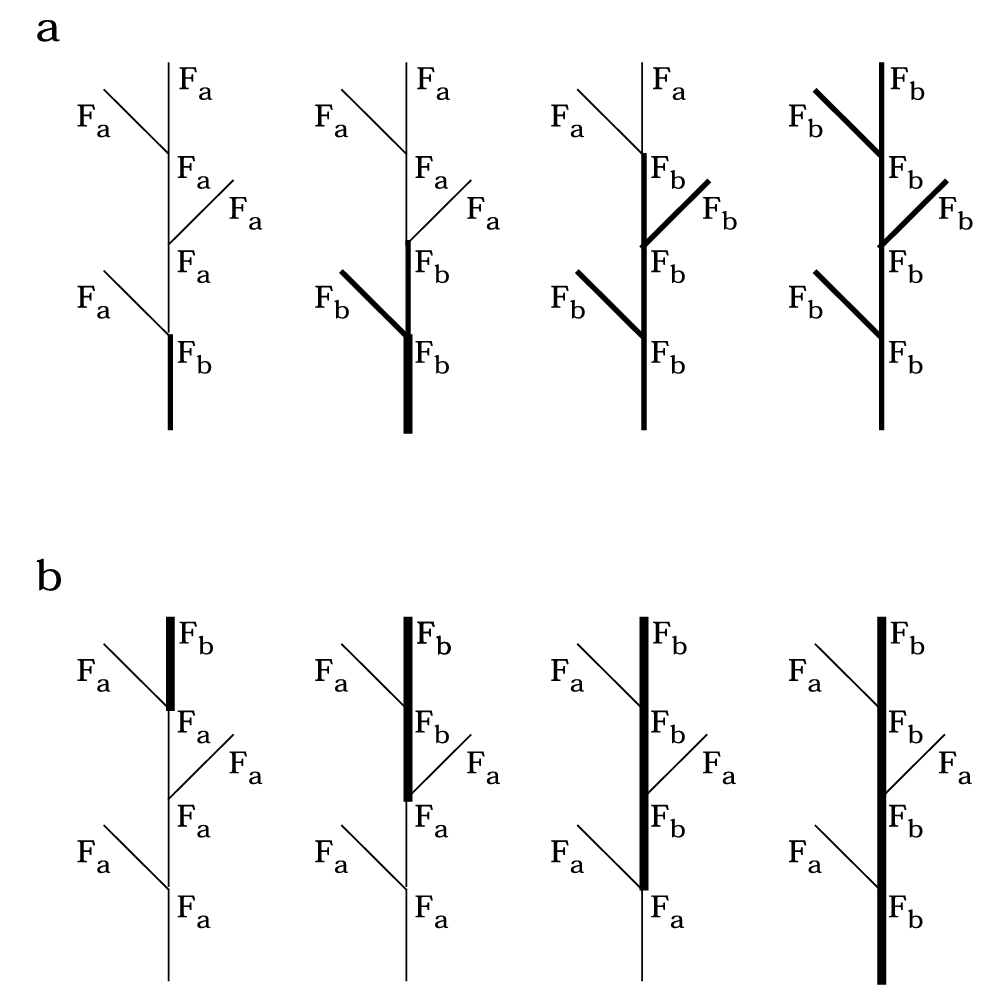
\includegraphics[width=12cm]{basic.png}
    \begin{minipage}[c]{13cm}
    \caption{\centering Signal propagation in a branching structure: (a) acropetal, (b) basipetal. Source:~\cite{PRU:1996}.}
    \label{fig:basic}
    \end{minipage}
\end{figure}

Within the concept of bracketed l-systems, the left context can be used to simulate control signals that propagate \emph{acropetally} | from the root or base to the extremities of the modelled plant | whereas the right context may represent control signals that propagate \emph{basipetally} | from the extremities to the base. We can take the following 1L-system that simulates an acropetal signal | without the tree growing | as an example and adjust it to also demonstrate the opposite as well:
\begin{center}
    \begin{minipage}[c]{5cm}
        $\# ignore:+ -$\newline\newline
        $\omega$: $F_b[+F_a]F_a[−F_a]F_a[+F_a]F_a$\newline
        \emph{p:} $F_b<F_a \rightarrow F_b$
    \end{minipage}
\end{center}
The character $F_b$ represents a segment already reached by the signal, while $F_a$ represents those segments that the signal has not yet reached. The $\#ignore$ keyword denotes characters that should be considered non-existent when context-matching as they do not concern generation, in this case those characters are $+$ and $-$. Now, to use this same 1L-system to simulate a basipetal signal, we can simply change $p$ while keeping the rest exactly the same:
\begin{center}
    \begin{minipage}[c]{5cm}
        $\# ignore:+ -$\newline\newline
        $\omega$: $F_b[+F_a]F_a[−F_a]F_a[+F_a]F_a$\newline
        \emph{p:} $F_a>F_b \rightarrow F_b$
    \end{minipage}
\end{center}
Visually, these l-systems will be produced as the trees in Figure \ref{fig:basic}. Image \verb|a| shows the acropetal simulation, while image \verb|b| shows the basipetal signal.

The operation of context-sensitive systems has been investigated extensively, one of the most significant contributions coming from Hogeweg and Hesper who published an exhaustive study of 3584 patterns generated by a class of 2L-systems defined over the alphabet \{0,1\}~\cite{HOG:1974}. Some of these patterns developed plant-like shapes that were then refined further by Smith using advanced computer imagery~\cite{ARS:1984}.

\subsection*{Parametric L-Systems}

The concept of parametric l-systems was formulated mainly to simplify the representation of continuous phenomena within a model. Parametric l-systems extend the original concept by associating each character with one or more real-valued parameters. In addition, the application of a production may be dependent on an associated condition. Parametric l-system production have the form:
\begin{center}
    \begin{minipage}[c]{6.5cm}
        $predecessor:condition \rightarrow successor$
    \end{minipage}
\end{center}
The real-valued \emph{actual} parameters appearing in the words correspond to \emph{formal} parameters represented by names of variables in the specification of l-system productions. A letter with an associated sequence of formal parameters is called a \emph{formal module}, and a sequence of formal modules is called a \emph{formal parametric word}~\cite{HAN:1992}. If $\Sigma$ is a set of formal parameters, then $C(\Sigma)$ denotes a \emph{logical expression} with parameters from $\Sigma$, and $E(\Sigma)$ is an \emph{arithmetic expression} with parameters from the same set. Standard rules for constructing syntactically correct expressions are observed, using the operator precedence and associativity presented in the table. Relational and logical expressions evaluate to zero for false and one for true. A logical statement specified as the empty string is assumed to have value one~\cite{PRU:1996}.

The graphic interpretation of parametric L-systems is similar to that of L-systems without parameters, except that characters used for drawing may be parametrized. For example, in a non-parametric L-system the character $F$ tells the turtle to move forward in the direction of the current heading by 1 world unit. A parametric L-system may contain $F(c)$ which indicates that the movement should be by $c$ world units. Other drawing commands behave similarly~\cite{HAN:1992}. 

Parameters can and have been applied to all the different l-systems. In the context of plant modelling, these allow for simulation of continuous natural processes like the constant development of branching structures or the diffusion of chemical compounds within non-branching microbial organisms. 

\section{Literature Survey}

I have gone through countless research papers based on and around L-systems to gain better understanding on the topic. Depending on the reason for research, the papers discuss L-system in varying detail with every paper citing the most significant sources: \emph{Algorithmic Beauty of Plants~\cite{PRU:1990}}, and \emph{Lindenmayer Systems, Fractals, and Plants~\cite{HAN:1989}}. The former is a book written mainly by Aristid Lindenmayer and Przemyslaw Prusinkiewicz, the latter is a volume of the Springer book series \emph{Lecture Notes in Biomathematics~\cite{SPR}} . Both sources have similar material, though where the book focuses on modeling and analyzing plant growth progression, the volume on lecture notes presents some other avenues as well. The book also goes into much greater detail about modelling specific plant systems and organs.

Some of the significant names come up quite frequently; Rozenberg and Salomaa~\cite{ROZ:1974}, Hogeweg and Hesper~\cite{HOG:1974}, and Hanan~\cite{HAN:1992} all made important progress that is still cited often in newer research. Rozenberg and Salomaa presented significant mathematical research into the functionalities of l-systems and are responsible for compiling two books worth of research from upwards of a dozen authors | The Book Of L~\cite{ROZAA}, and L Systems~\cite{LILA}. Hogeweg and Hesper published a study of countless patterns generated by 2L-systems that others then refined or expanded on. Hanan worked with Prusinkiewicz on ~\cite{HAN:1989}, and his PhD dissertation explores parametric l-systems in great detail in various contexts.

% CONSIDER TALKING ON GRAPHICAL INTERPRETATION

Majority of papers using L-systems in different kinds of research begin with D0L-systems and then proceed to more complex applications by adding context-sensitive aspects. The papers all use somewhat algebraic notation to define L-systems and provide \emph{proof}, though these notations are not ones I understand quite so well yet. Those considering mathematical proofs, do not always compute graphical demonstrations, although the theories of those proofs are occasionally seen in use elsewhere. 


\chapter{Design and Software Engineering}

I attempted to approach this project with something similar to an agile methodology, but quickly realized that it would be best for my way of working to focus on having only a final release with all major functionalities. It allowed me to focus on getting multiple examples of each kind of l-system while also refining my program as necessary with the changes.

Research on l-systems gave me several ideas of how to approach this project in terms of code deliverables. Among the many implementations of l-systems I found, very few were executed in Java. Despite this, I could take inspiration from several places on where to begin. There are countless examples available online for the actual axiom and rules for existing l-system fractals and trees | most of them extensively researched and developed | but for the actual coding, I took guidance from \emph{The Nature of Code}~\cite{NOC:2024}.

% Basic overview before going in depth
\section{Program Structure}

I had already decided that I wanted to utilize object-oriented programming, and I could very clearly separate the objects I needed by their function. The implementation of L-systems requires a way to rewrite strings according to the rules corresponding to specific characters, and a way to translate the resulting strings into graphical output. 

The main defined objects are:
\begin{itemize}
    \item a \verb|Rule| object
    \begin{itemize}
        \item stores a character and its corresponding production string
        \item a second constructor separates stochastic and non-stochastic rules; stochastic rules contain an outcome probability as well
        \item contains getters for all attributes to be called in \verb|LSystem|
    \end{itemize}
    \item an \verb|LSystem| object
    \begin{itemize}
        \item initializes with an axiom and a \verb|List| of \verb|Rule| objects, a \verb|Boolean| defines whether it is stochastic or not
        \item contains a getter for the sentence as that is the only attribute accessed outside of the object and is only updated within the class
        \item checks if a character has a production rule corresponding to it
        \item creates deterministic generations by rewriting the string using the rule set
        \item creates stochastic generations using a randomized function according to the ruleset
    \end{itemize}
    \item a \verb|Turtle| object
    \begin{itemize}
        \item initializes with a length and angle value corresponding to the specific L-system it is made for
        \item translates the LSystem string passed through to it into graphical output using Processing commands
    \end{itemize}
\end{itemize}

The main executor for this program is a class | \verb|Sketch| | extending \verb|PApplet|, which is the Processing class used to create interfaces and simulate interactions. Implementing \verb|PApplet| in Java requires overwriting the default functions to execute properly: \verb|setup()|, contains initializing of \verb|PApplet| as well as all objects that will be used as this code executes only once at the begining; \verb|settings()|, contains settings for the output window such as size of the window; \verb|draw()|, contains all code required for the window output.

\begin{figure}[h]
    \centering
	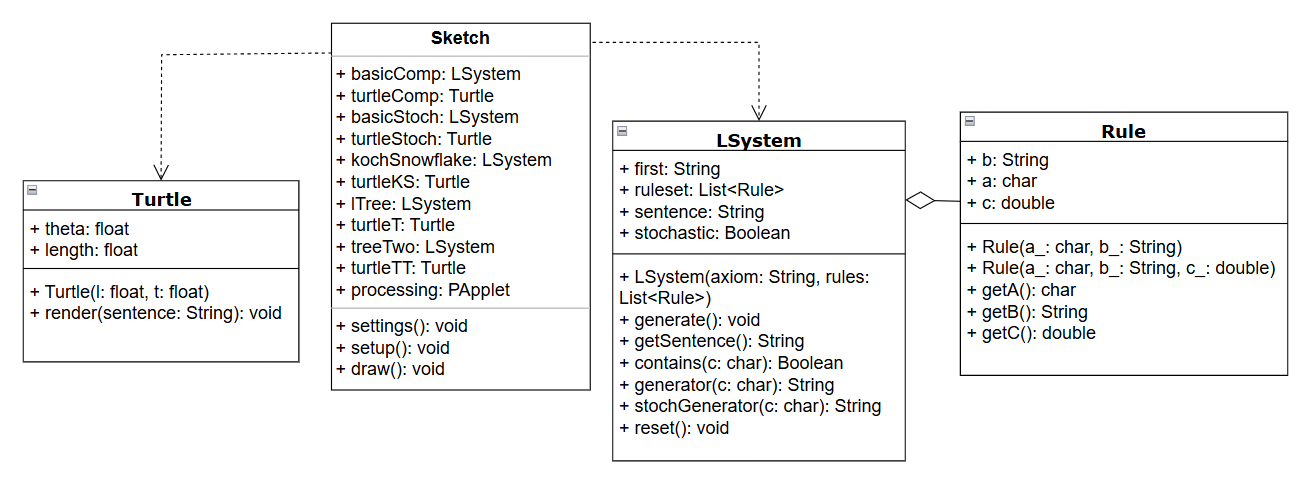
\includegraphics[width=16cm]{FYP_UML2.png} 
    \caption{\label{fig:finalUML} UML diagram showing relationships between classes.}
\end{figure}

All objects are defined within \verb|Sketch|. I wanted each of the objects to have isolated functionalities, so every l-system image exists within its own defined object, has its own \verb|List| of \verb|Rule| objects and its own \verb|Turtle|. \verb|Turtle| only consists of output commands, \verb|LSystem| holds only l-system encoding including the generators and rule confirmation functions, and \verb|Rule| only holds the rules with their probability of outcome where necessary.  The UML diagram provided shows all the classes and the relationships between them.

\section{Implementations of Significance}

\subsection*{\texttt{Turtle.render()}} 

The LOGO turtle that this one is based on has very straightforward commands, however they obviously are not associated with specific characters.  The nature of the execution required strings that exist within a compact form as in a single character defines a complete command. This method defines specific commands for each drawable character. 
\begin{verbatim}
        switch (c){
                case 'F', 'G':
                    Sketch.processing.strokeWeight(2);
                    Sketch.processing.line(0, 0, 0, length);
                    Sketch.processing.translate(0, length);
                    break;
                case '+':
                    // rotate right
                    Sketch.processing.rotate(theta);
                    break;
                case '-':
                    // rotate left
                    Sketch.processing.rotate(-theta);
                    break;
                case '[':
                    // saves branching off position
                    Sketch.processing.pushMatrix();
                    break;
                case ']':
                    // returns to branching off position to continue drawing from there
                    Sketch.processing.popMatrix();
            }
\end{verbatim}

The method loops through the \verb|String| passed through as a parameter, drawing according to the characters that have commands corresponding to them. No change is enacted for unrecognized characters because extra characters are sometimes used to apply certain kinds of rewriting behaviour. Due to the nature of Processing \verb|core.jar|, every Processing function that is called needs to reference the instance of \verb|PApplet| that exists in \verb|Sketch|. I attempted to import and initialize \verb|PApplet| within the \verb|Turtle| file, but this was not possible so had to reference it as \verb|Sketch.processing| with every function.

\subsection*{\texttt{LSystem.generate()}}

This method calls a generator inside a loop that cycles through the entire sentence. Which generator is called depends on the Boolean \verb|stochastic| that is initialized in the constructor. An \verb|if| statement determines whether the Boolean is true or false, and the execution lies with that and the \verb|else|. I did consider having the condition inside the loop but realized immediately that the sentence would likely be increasing exponentially and it would be completely unreasonable for it to go through the condition statement for every character when it will remain unchanged. The rule string is appended to a \verb|StringBuilder| which is then used to update the local \verb|sentence| variable.

\subsection*{\texttt{generator()}}

While fairly standard in terms of cycling through a \verb|List| and returning the rule corresponding to a specific character, I wanted to mention this function to compare with the \verb|stochGenerator|. If a rule is not found for the character, the function returns null.
\begin{verbatim}
        for (Rule rule : ruleset){
            comp = rule.getA();

            if (c == comp){
                return rule.getB();
            }
        }
        return null;
\end{verbatim}

This \verb|generator| is only used if the l-system is non-stochastic since those systems have one rule for every unique letter in the alphabet. There is no concern with these about probabilities or multiple rules.

\subsection*{\texttt{stochGenerator()}}

The stochastic generator is a bit more complex in terms of execution. I had some trouble figuring out how to implement generation dependent on probabilities but eventually, I found a method of execution that fit with suitably with my code structure~\cite{CTR}. I first cycle through and add all the strings related to a single character in one \verb|ArrayList| and all the probabilities connected to them in another. 
\begin{verbatim}
        Random random = new Random();
        Double cumulativeProbability = 0.0;
        double randomVal = random.nextDouble();

        for (int i = 0; i < strings.size(); i++) {
            cumulativeProbability += probabilities.get(i);

            if (randomVal <= cumulativeProbability) {
                return strings.get(i);
            }
        }
        return strings.getLast();
\end{verbatim}

In the code snippet, \verb|randomVal| is a random generated value between \verb|0.0| and \verb|1.0|. A cumulative probability sum is calculated incrementally, and when the random value is equal to or less than the cumulative, the corresponding string is selected to be returned. In the case that no string is selected within the loop, the last string in the \verb|ArrayList| is selected to be returned.

\section{Experimenting with GUI}

 Due to the way in which I have coded \verb|Turtle| and the way that \verb|draw()| works in Processing, the images are generated all at once and the window opens with all the generations already ready. Despite looking into the documentation in great detail, I did not understand how to make the window show its drawing progress until very close to the submission. Once I did, I realized I would have had to redo \verb|Turtle| almost entirely so decided to leave it be. 

\begin{figure}[h]
    \centering
	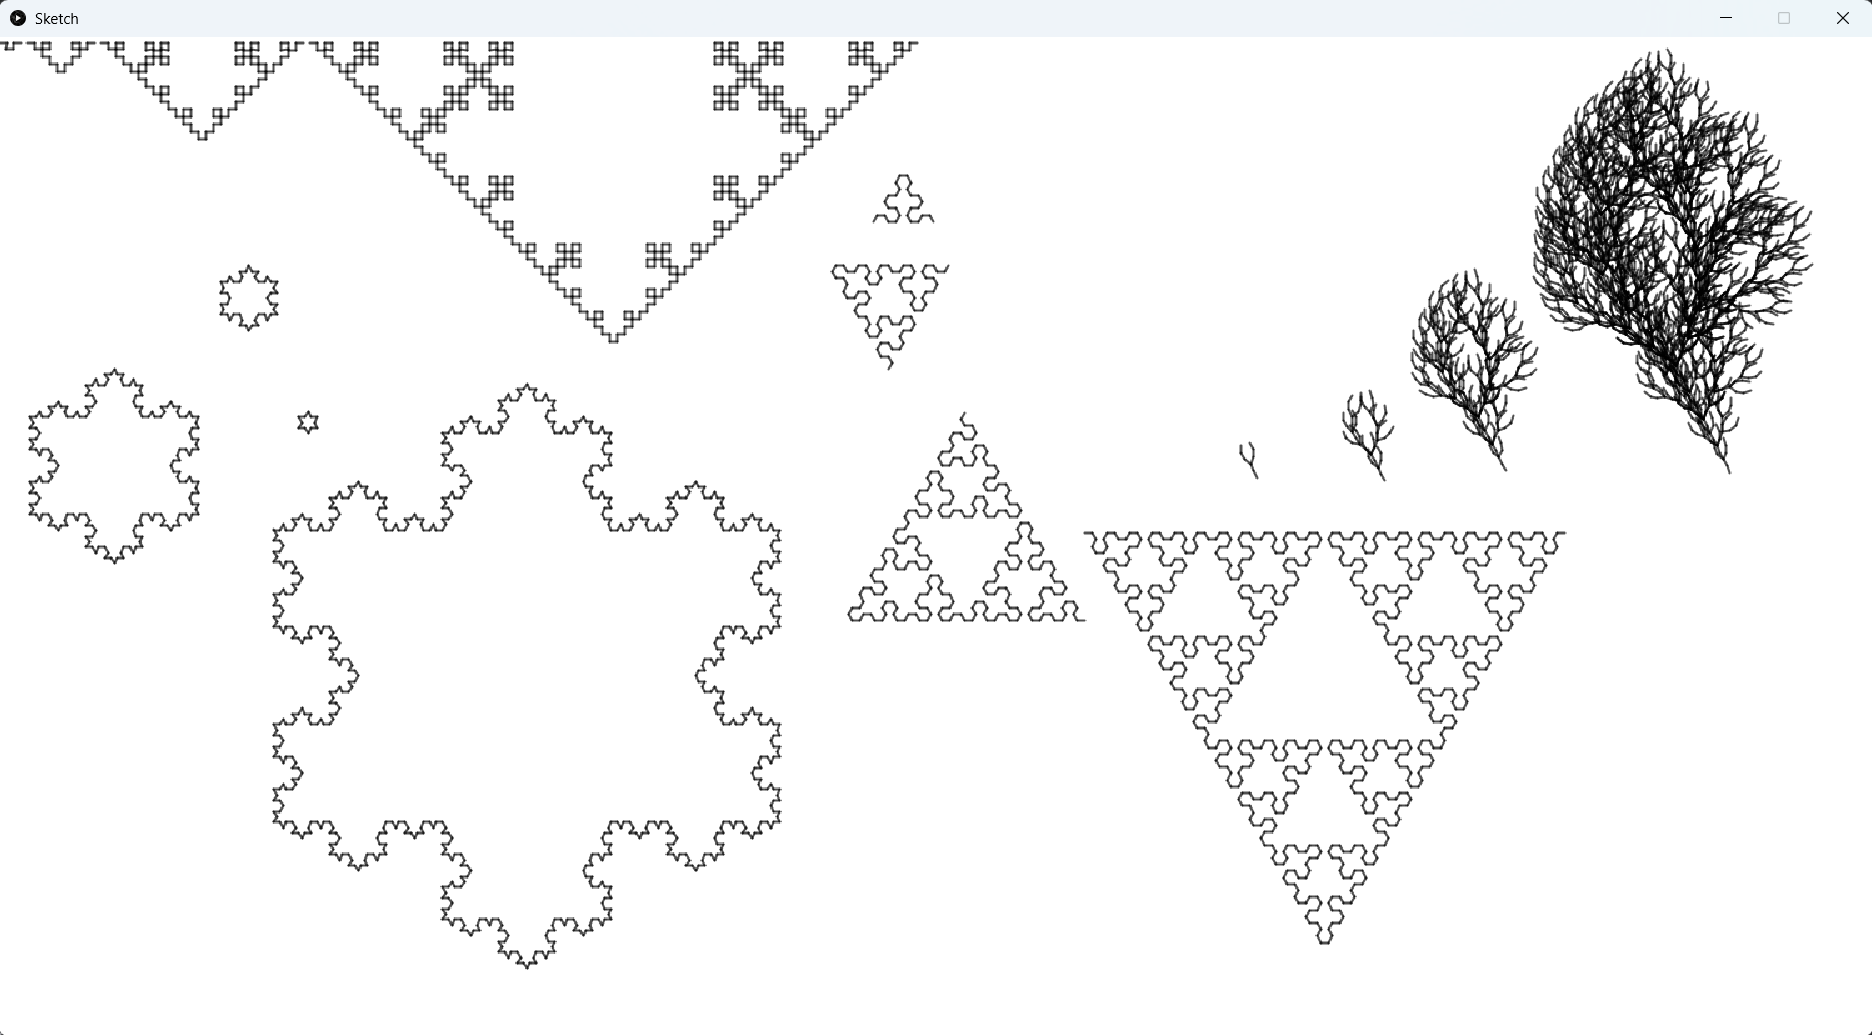
\includegraphics[width=15cm]{firstOutput.png} 
    \caption{\label{fig:image} Output from initial implementation.}
\end{figure}

The above figure shows the output window from my interim submission. Since I couldn't get it functional, I wanted to at least have enough examples that it showed the variations in image generations that I wanted. The images starting from top left and going anti-clockwise are: quadratic Koch curve, Koch snowflake, Sierpinski triangle, a D0L Tree.

In Term 2, I started working on stochastic systems and, eventually, began attempts with a more sophisticated GUI. My first attempt was with G4P~\cite{G4P}, a library developed by an independent programmer. The documentation while extensive was confusing to navigate and with the recommended GUI Builder tool not functioning with IntelliJ, I felt discouraged in trying to use it in the project. 

I then attempted to use LazyGui~\cite{LAZY} since it promised to be simple to use and had implement instructions for IntelliJ in its ReadMe. The code and documentation was easy to understand and the trial implementation was straightforward and successful. Integrating the \verb|Sketch| code, however, brought about some complications. My approach in integration was to add the basic LazyGui setup to the Sketch layout with all the Turtle code commented out to evaluate basic function. It remained unresponsive. I tried multiple ways of initializing and structuring, but the code refused to even compile, so I abandoned that as well. With how close the deadline of submission was, I decided to focus on functionality and resigned to just the default Processing library of \verb|PApplet|.

Due to time constraints, I resigned myself to having a very basic end result. I did try to continue still, with an attempt at using the l-system example code Processing has available on their website. It turned out disastrous after I changed the colours since I wanted black on white, instead of the default white on black. The code had the line colour set twice despite there being no necessity for it. The redundant code had me frustrated after I spent hours trying to understand why there was no image being produced despite the code running. I resorted to adding \verb|System.out.println| statements in different sections bit by bit to find the problem. Needless to say, I will not be making the same mistake again.

\begin{figure}[h]
    \centering
	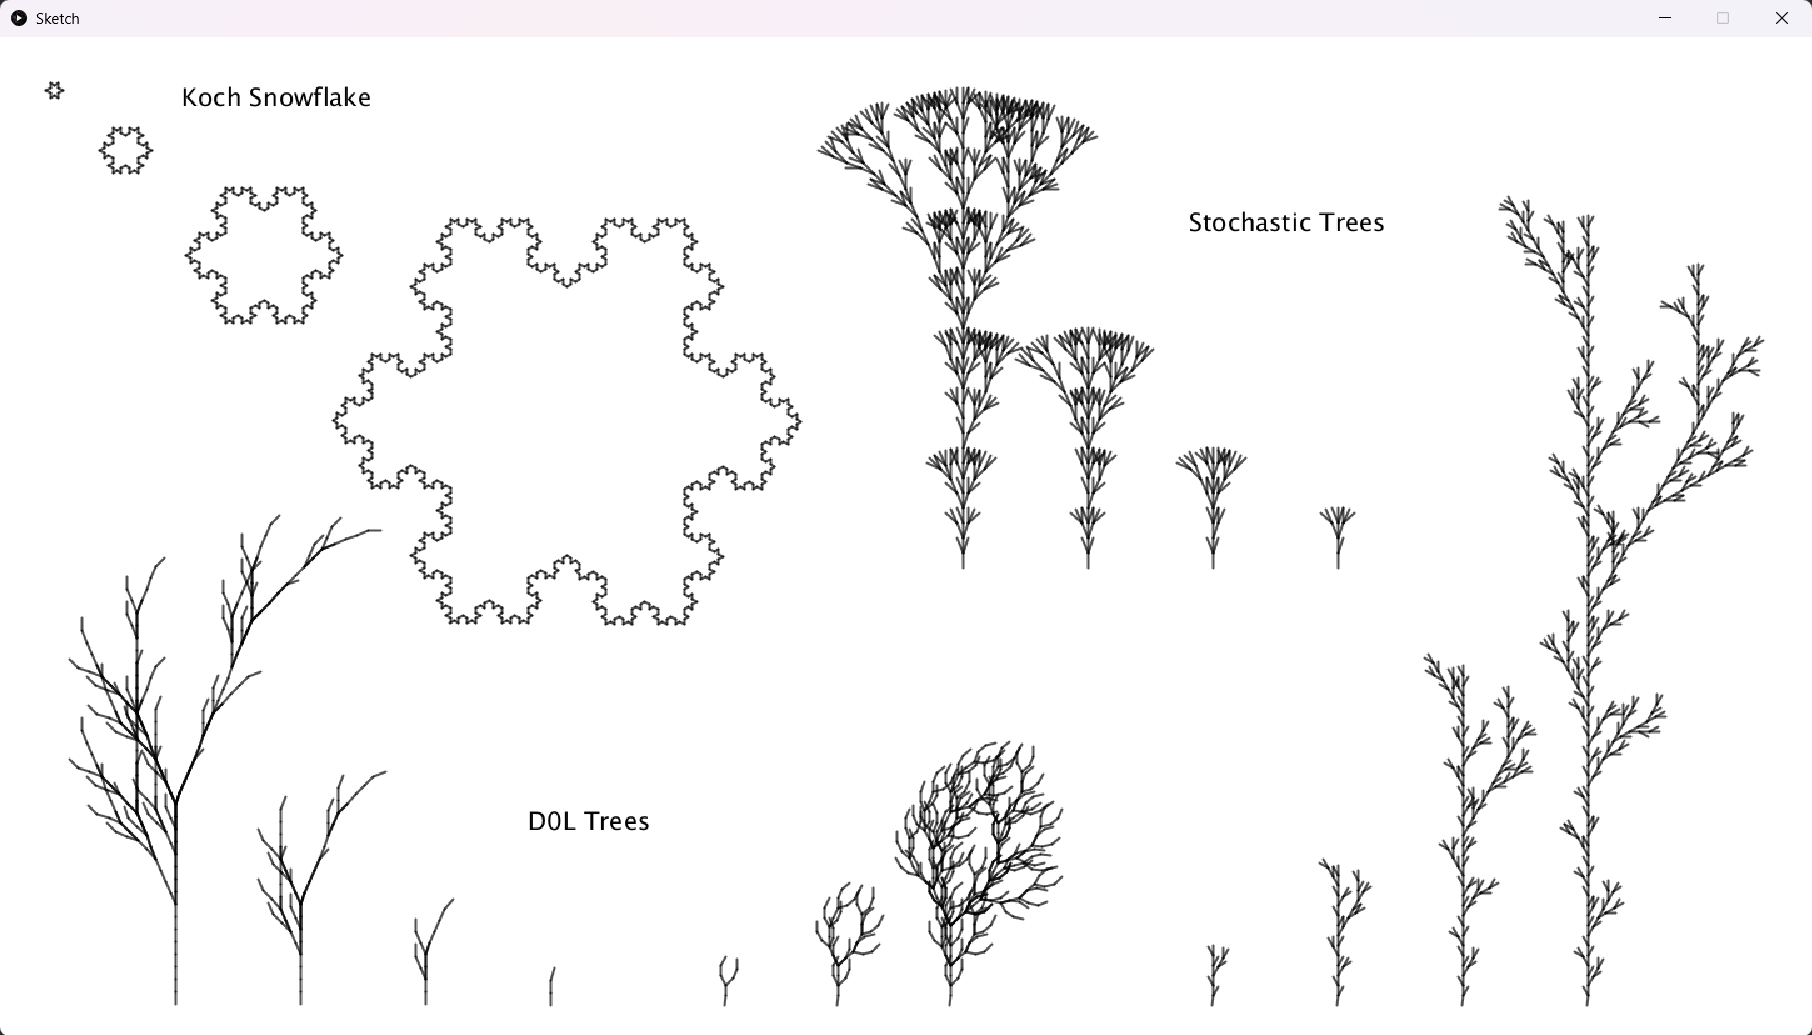
\includegraphics[width=15cm]{Stochastic.png} 
    \caption{\label{fig:image} Output from final implementation.}
\end{figure}

Since I had no guarantees that I would be able to restructure \verb|Turtle| as required for any kind of complex execution, I focused on providing functional stochastic images instead. The above shows my final output window. I found a way to have the stochastic trees refresh and redraw, and set the frame rate to 0.8 to have the trees change every 1.25s. This allows the observer to see how the stochastic productions vary despite all conditions remaining unchanged.

\section{Technological Choices}

The initial implementation was accomplished using the \emph{Processing 4.3}~\cite{PRC} core library. This was selected due to its straightforward implementation of drawn graphics as well as the convenience of adapting its functionalities to the project's needs. The commands required to control output on a window are highly similar to traditional turtle graphics, a method used in most 2D implementations of L-systems and also the one depicted in the original sources~\cite{PRU:1990}~\cite{HAN:1989}. Using Processing with a defined \verb|Turtle| object | to account for the variation in line length and angle values | allows for easier generation of fractal images that have been previously defined, using notation corresponding to turtle commands.

There is, however, an issue that arose with the use of Processing. Since Processing exists as an IDE with its own language that is closely based on Java but is still distinct in itself, the use of its core library in a Java program was not as simple as it initially appeared. Almost all resources of Processing make use of or reference it as an IDE, so adapting related libraries and tools to this implementation required some maneuvering. For example, I could not import \verb|PApplet| to my \verb|Turtle| file despite needing features from it in that class. I instead had to reference the \verb|Sketch| class and the \verb|PApplet| initialization in there for every \verb|PApplet| function used. This was a simple issue, though, since it was fairly straightforward and easily resolved.

Not all functionalities outside of the default proved to be as effective or easy to manage, however,  and several of the libraries I was planning on using for advanced UI implementation ended up being incompatible with the current version of Processing. Despite the libraries still being listed on the Processing website, several of them are no longer supported. Outside of those, G4P uses a tool that was incompatible with my IDE and I could not account for it since I got to that point of implementation later than expected. LazyGui | while it appears to be supported and regularly updated, and has capability of use in IntelliJ | did not work for my code despite extensive attempts at debugging.

\section{Git Usage}

I made use of branches to keep parts of the project separate. My \verb|diaryUpdates| branch has only diary entries. I did consider this to be a step too far initially, but it proved convenient for me because it forced me to complete my ongoing work and have a useful commit before I switched to write down my thoughts and progress reports. The \verb|fractals| branch has all the main implementation of D0L-systems. A testing branch kept the tests and any edits made on that branch separate in case some error arises from the editing. I did, on occasion have to fetch files from different branches, namely the LSystem file from the testing branch after errors in the code were fixed. 

My Term 2 implementation saw me making use of a separate for the stochastic productions | \verb|stochasticImp| | so I could clear all code for the deterministic systems and start working on the randomness with as much of a blank slate as possible. I kept all the files apart from Sketch intact since that code was mostly used as is, apart from the addition of two functions. It also allowed me to pull the necessary fractals from \verb|fractals| once my implementation was complete. 

I did also use separate branches for my GUI attempts. I was planning on having a separate branch for \verb|lazyGuiTrial|, but the GUI Builder tool used for it was incompatible with my set-up so I did not have any useful commits from it and simply changed the name of the G4P branch to use it for lazyGui instead. I am very thankful for having a separate branch for this, though, because when my attempts with lazyGui were as unsuccessful as they were, I could simply switch back to \verb|stochasticImp|, and begin anew with a different framework.

I made the \verb|reportFigures| branch simply because I did not want the structure of my final code to be affected when I was trying to get specific images to add to this document. The \verb|processingExTrial| was an attempt to see the function of the default Processing features; I cleared all code to copy paste the example code available on the website, mostly to see what was functional and what was not.

\section{Testing}

I tried my best to be systematic with testing for the length of this project, but most of my testing turned out to be a manual running and rerunning of my program due to the graphics used. I tried to find a formal testing strategy for Processing, but was unsuccessful. There is no formal testing for Processing programs, whether related to JUnit or otherwise. I did find an entry on the Processing forum asking about unit testing~\cite{TEST}, but it had nothing posted that helps test the features of my project.

The only files for which JUnit tests could be carried out, were \verb|LSystem| and \verb|Rule|. For these tests I created a separate branch, \verb|testLString|, where I initially only tested the \verb|getSentence()|, \verb|generate()|, and \verb|contains()| from \verb|LSystem|. For \verb|contains|, I tested using both true and false values. I did previously have another function \verb|valid()| | which I removed after extending for stochastic implementation | that I had also created tests for but removed once the method was no longer part of my implementation.

After my stochastic implementation in Term 2, I did add tests for one of the new methods, \verb|reset()|, and realized that I did not have any tests for the \verb|Rule| class despite it having get functions. I added tests for the normal getters and tested the second constructor that was developed for that class along with the additional getter for the probability value. I did try to add a test for my \verb|stochGenerator()|, but due the nature of its random generation I was not able to write something that tested it well. I instead used the fact that the visual generations were different every time the window refreshed as confirmation that it worked correctly.

The \verb|Sketch| and final image generation was tested by running and refreshing the window as necessary. I needed to do this to position the figures right so that they could be seen clearly and with minimal to no overlap. This also allowed me to see the stochastic productions as previously mentioned, the differences in images proved not only that \verb|stochGenerator| was functioning correctly, but also that the window was refreshing on the mouse click as expected.

\chapter{Professional Issues}

It is important to consider issues that might arise during the process of working on delivering a complex product and then reflect once again upon achieving the results. With a project so rooted in the demonstration of an intricate concept, it must be taken into account how easy to understand and navigate the end product is. If a project is lacking usability, it is unlikely to leave a positive impression on the user of your product the way you want. Difficult to handle programs that lack intuitive structure and convenient features are going to discourage recurrent use of and interaction with the program. 

When it comes to educational programs such as this that attempt to present a new, complicated topic to a user that has no prior knowledge of it, the end product should encourage interaction from the user. Interactive aspects in a program make it interesting to open and run.  The objective must be to nurture curiosity and teach, which is only made easier by having a program design that does not confuse the user. With the current economy being where it is, it is highly common to see bright, popping adverts even on educational sites or in educational applications and programs that not just distract but actively push learners away from intellectual endeavours. When educators or developers stop considering accessibility and usability, they make their products difficult to use and prevent learners from seeking them out.

 In a university project, where every aspect of the submitted product is likely to be analysed for utility and usability, it is important for a student to be able to demonstrate the skills required for such a thing. It shows the student’s attention to detail and the considerations they must have taken when planning and working on their project. This leads into a major issue I had to deal with in the build process. An objective that was set from the beginning, both by myself and the project requirement, was a functioning interface that could demonstrate skills I had worked on. I approached Processing highly optimistic. It is a learning tool that is easy to use and manage work in. Another positive; it already has libraries published by independent developers to allow users to implement advanced GUI elements. 

I planned out my approach to it from the start, making sure that I didn’t forget what libraries I was considering and which ones I had counted off already because of usability or because I was simply unable to find documentation. Upon reaching the UI development phase, I found that the main library I had been considering was no longer supported and had not been compatible with several of the newer versions of Processing, including the version I was using. The information about it being unsupported or incompatible was nowhere to be found. I only discovered this after I could not find the correct imports necessary and went through a discussion on the Processing forum. It is important to note that these libraries are listed on the Processing website together with the ones that are supported and compatible but with no indicator of either fact. 

This raises an important point of discussion about reliable software, especially as a platform encouraging experimentation and independent discovery. It is quite common in computing to come across software and software features, or websites and other once valuable resources that are no longer supported and have no warning or identifier alerting users to the fact. In cases such as this, it dramatically affects the capacity of a user to be able to expand their work to the level they strive for. In a university setting where not only are students working on limited time but are also being evaluated on their final presentation of skills, it can significantly stunt their growth as developers. The limited time prevents repetitive trial and error, and even in instances where there is time, only so much of it can be dedicated to one aspect of a much larger project.

In a harsher environment, this issue of unsupported software can be extremely harmful. Unsupported software and server products have the potential to create vulnerabilities without the user being suspicious of anything amiss. The NCSC says, “All software, including device operating systems, will eventually become out of date. Ideally, once out of date, technology should not be used.”~\cite{SEC} Using unsupported resources or even resources that are not \emph{sufficiently} supported can raise major problems. A well-known example of insufficient support increasing vulnerability can be seen in Heartbleed bug~\cite{HEART}. OpenSSL was being managed by 15 active developers when the issue arose from the code additions of an independent contributor. The vulnerability affected 17\% of all SSL servers and countless major companies were affected by the bug. The incident forced a conversation about better support and funding towards cybersecurity and prompt responses. Despite all this, some enterprises neglected patching and as recent as 202, there were still hundreds of thousands of computers found vulnerable still. 


% USABILITY DEFINITION
% IMPORTANCE OF USABILITY OF END PRODUCT
    % FOCUS IN REGARDS TO UNIVERSITY PROJECT
    % DEMONSTRATION OF KNOWLEDGE AND SKILLS
% IMPORTANCE OF UPDATED RESOURCES
    % ISSUES RAISED DURING TIME CONSTRAINED PROJECTS
        % TIE IN TO UNIVERSITY PROJECT
        % COMPROMISES DEMONSTRATION OF TRUE CAPABILITY 
    % CLEAR SEPARATION OF VERSION COMPATIBILE RESOURCES VS INCOMPATIBLE
    % EFFECT ON USAGE AND RELIABILITY OF ADVERTISED RESOURCE
% SOCIETAL RESPONSIBILITY
    % ACCESSIBILITY ACROSS DEMOGRAPHICS
% CITATION AND ACKNOWLEDGMENTS
    % FOCUS ON USE OF CODE AND FIGURES FROM INDEPENDENT SOURCES
% BALANCING EXPECTATIONS
    % FOCUS FOCUS ON SMALLER GOALS INSTEAD OF TRYING TO PUSH AHEAD BEFORE DONE WITH CURRENT PROBLEM


\chapter{Conclusion}

L-systems have extensive uses across countless fields. While it is seen commonly within research, it has also been developed extensively for use in art and music. This report has presented some of the significant classes of l-system, highlighted differences between certain kinds, and discussed the way in which they present output and are utilized for research. While the broader goals of the project have been achieved, some of the more specific aspects of GUI did not reach the level of functionality or complexity that were aimed for. Though the execution did demonstrate the variations between stochastic and non-stochastic l-systems and their outputs, which has been a significant aim since the beginning.

\section{Self-evaluation}

Overall this has been an incredibly interesting topic to research. In looking into l-system classes and reading through research across seemingly unconnected areas, I have had my eyes opened on just how much overlap exists between various academic fields especially with the development of specialized tools. For the main types based research, I did have to filter through the same small pool of authors, majority of the publications being from before the turn of the century, but the research still proved incredibly intriguing and was amongst the most enjoyable parts of my project.

It is very easy to generalise issues of time management and I have mentioned them previously regardless, so I will focus on the sections of the project that proved less successful or could have been improved.

I have discussed the trouble I faced with implementing a proper GUI, but my implementation of the turtle is something that significantly held me back on producing an animated window as well. Despite the research and experimentation with code, I did not realize until too late what was keeping me from achieving the effects I wanted out of Processing. With earlier understanding of my tools, I would have been able to produce a more advanced end product. Regardless of the outcome, I am satisfied that I explored what I could in the time I had available. I experimented with three different GUI implements, which while unsuccessful, taught me how to alter my approach to projects like these in the future. I also believe that my presentation of the l-system images themselves came out neat and the different classes implemented remained clearly discernible.

One thing I have noticed that cause quite a bit of trouble for me is my tendency to focus on one medium at a time. Once I shifted focus to research and research papers, I practically forgot that video tutorials could have helped me significantly if I had remembered them in time. Even with the separation of using the Processing IDE and using Processing \verb|.core| with Java, I could have found guidance and understanding of the functions and how they work. I tried my best with the resources I did use however, and found a way to animate the window so the user could see the variation of productions without needing to do anything.

My progress over Term 2 was tedious, and I ended up with a gap where little could be done to extend my code and research had gone slower as well. I had some hardware issues at a very crucial time where my laptop cursor would spontaneously stop responding or disable itself without reason. It took a few days to resolve entirely since I would fix it and then have the issue pop up again in a few hours time or the next day. It was a new problem, not an issue I expected to be dealing with. Overall, I know what I need to improve in my approach with long-term projects like this, and will be making an effort to enact changes in my professional life going forward.

\section{Future Work and Extension}

I mentioned the main things that had me interested and eager to work on this project in my motivation section and I wanted to make note of some possible extensions for the topic and program I have developed so far. I have quite a few ideas for the actual l-system executions, but my focus for a while will be on building the GUI that I had imagined. I have a better understanding of Processing now and, without a time constraint, would also be more confident exploring the potential incorporation of JavaFX into the project to have something more navigable. 

With the basis of l-system generation set up, I have enough understanding of the concept to be able to apply it in other languages or using other frameworks. I believe that being able to code familiar concepts in different languages helps hone skills and increase comfort with languages that a user might be feeling rusty in or might want to learn anew. This would be a good concept for coding exercises since it is easy to start with a simple implementation and then continue expanding until the desired complexity or functionality is reached; starting with D0L-systems and expanding on the exercise until coding in newer languages is second nature. I have also considered expanding this into 3D development. While I have used resources such as Blender in a more casual artistic context, I know it contains scripting functionalities. It would be interesting to look into implements like this, allowing me to gain skills that I could continue to utilize elsewhere as well. 

I also have some curiosity about "regeneration" in terms of l-systems. I found mention of some considerations of the concept in \emph{Developmental Systems and Languages}~\cite{LIN:1972}, but it was only mentioned in passing. What I understood from the brief mention was that it followed the concept of regenerating limbs and regrowing a plant from a cutting of it. The logical assumption being that segments of these kinds of strings should also be able to \emph{regenerate} in the same way. While I haven't looked for research specific to this concept, nothing similar came up during my general research that caught my eye or sounded anywhere similar to this, so I wonder how much this regeneration theory was explored in practice. I wonder if there is a way to implement some sort of "memory layer" to a model to enact regeneration, or perhaps isolate a segment of the l-system from the rest to apply production rules to; all this while making sure that the inherent nature of l-systems remains unchanged. Needless to say, I have a lot of theories I wish to explore in my own time.




\chapter{Appendix}

\section{Diary}

\textbf{Lindenmayer Systems Project Diary}

Entry 23 - April 13th

Changed the comparison stochastic tree to a different one, so there is evidence of two separate systems showcasing stochastic rewriting. Shifting my focus to report work entirely until I can meet with my supervisor and discuss the GUI issue. I have some papers that I want to integrate into my report - I've noted these in my written diary - and some restructuring is required. I want to separate the research section from the implementation a bit more clearly. I am considered having some examples of other classes of L-Systems as well, maybe n a different branch, so I can use the output in my report since I don't have space on the overall output window. I will leave that for last, possibly until after everything else is completed and signed off by the supe.

Entry 22 - April 11th

I went back to the website-given examples to debug a bit. Managed to figure out the issue, and it was a really minor code change. The line colour is initialized in the setup() and I assumed that they would not have it mentioned again as that would be redundant, but the whole time that I had switched the background colour and stroke colour (since the examples were white stroke on black background and I wanted the opposite), they had reiterated the stroke colour in the second file. The program was drawing white on white. Two days I spent trying to understand why it wasn't functioning. Also realized that I was having so much issue with adjusting my productions on the window because I wasn't converting my angle calculations into radians. I added a reset function to LSystem which redraws the entire setup I have exactly, so that the difference in stochastic productions can be seen with every click. I did consider restructuring my work (again) so I could replicate the actively drawing visuals that the website examples manage, but I don't know how compatible that is with my code. I'll consider it, but until then I will be switching out the basicComp tree for a different stochastic system. That would give me more visibly different examples to showcase. I did readjust my output window, so now I have one geometric fractal, two deterministic trees, and two stochastic trees. I need to remove the tests that used valid().
For report reference - added a reset() function, removed the valid() function. Thought process in written diary.

Entry 21 - April 10th

I don't know how to approach the GUI issue anymore. I've worked on and implemented a stochastic L-system. With the current setup not having a navigable interface, I will have to remove some of the fractal productions so that there is space on the initial window to also hold the stochastic productions. Haven't figured out how exactly to set that up, but will work on that next. I've been considering how to take and use keyboard inputs to maybe maneuver something GUI-adjacent with that instead. It is clear that I am unlikely to have a properly traversable interface, but I can still try a basic input-output concept.
For report reference - the probability consideration with selecting outputs came from codingtechroom, and the example used is already in the report theory (mention again in software engineering section?)

Entry 20 - April 9th

I attempted to look at my problem a different way. I will be abandoning the LazyGui branch as I don't think there's anything else I can do with it if the most basic output isn't working. During my initial research I had found the L-System examples given on the Processing website, but I kept myself from using them as I had planned a slightly different approach, separating drawing and rewriting functionalities between the Turtle and LSystem objects respectively. I decided to use the examples provided on the website and spent all of yesterday implementing those on a separate branch to see if those would be functional with my setup. They were not. I separated the files the way the examples had them separated; still to no avail. Using the example code exactly as it is, creates a window with a background, but none of the actual drawing occurs.
For report reference - pentigree, snowflake, and penrose L-systems, all by Geraldine Sarmiento. Copied word-for-word to see if they worked and if so, to what extent.

Entry 19 - April 7th

Went back to refining my report. I worked on the software engineering portion since I appear to have reached a standstill with my code and need a break before returning to it.

Entry 18 - April 5th

I have been attempting to work with LazyGui, but it is not proving very effective. I attempted to begin with the most basic code for it to get an idea of whether it would even be functional and it did. It worked for a simple output. I decided I would begin slowly integrated parts of the actual graphical output from there but nothing I try is working with my code setup. I have used the IntelliJ-specific examples given by KrabCode, the author of LazyGui, with no success. While the initial attempt proved functional, I have seen no progress since. I have attempted multiple different ways of implementation, going so far as to restructure part of my code, but I am stuck with a consistent error that keeps the code from running. At one point I got it to create a window, but it would still not create a render, only a blank window. It is so late into the process to make significant changes that I am hesitant to stop trying and move to yet another GUI framework. I will be back at step 1 again no matter what framework I switch over to. I will keep trying for at least another day or two then reevaluate. I understand that I shouldn't have taken such a risk so late into the timeline, and I am struggling a bit with what could have gone differently if I had made different decisions, but I need to work on now with what I have.

Entry 17 - March 22nd

I've been making additions to my report. I have not had a significant amount of time to work on the code due to multiple coursework submissions being very close together. I have continued working on Overleaf for my report as it remains the most convenient option for me. Additions to the report so far consist of the report-based deliverables discussing some further classifications of L-Systems I found in a research paper from a Springer Archive book Lindenmayer Systems: Impacts on Theoretical Computer Science, Computer Graphics, and Developmental Biology. The information is spread over a variety of topics, so I have had to go back and forth between a couple papers to understand which classifications are truly distinct and which ones overlap enough to disregard.

Entry 16 - March 15th

I've been trying to produce a functional output as I want with G4P which is proving unsuccessful and not all the way compatible with the version of Processing that I am using. Exploring options once again with LazyGui, another library created for Processing. This one has more recent updates and appears to be compatible with Processing 4 and the readme includes some reference to integrating it into IntelliJ which I'm hoping means that I can implement it without too much trouble.

Entry 15 - March 9th

After changing absolutely nothing in my code apart from writing it out in front of a friend, the Processing redraw function worked flawlessly, triggered by mousePressed which also did not work previously. I feel like I can't progress with JavaFX now. It feels like an insane drawback but if it works then it's a much more reasonable progression to stick to one library instead of integrating three separate things that aren't commonly or easily used together. This may affect the timeline but I'm behind anyway so I'll make up time where possible.
This is frustrating and I feel like all the time I've spent trying to make Processing work has been wasted because the very first method I tried is now functional despite no change to the rest of the code. Keep calm and carry on, I suppose.

Entry 14 - Feb 28th

I've not had a very productive month in the context of this project. I'm going to begin shifting to JavaFX from now. I plan to work on some base stochastic implementation before that, so I at least have something to show with the Processing sketches still. The issue with continuing with Processing now is that G4P and its corresponding GUI Builder were created with the Processing IDE and its specific language (similar to Java but ultimately different) in mind. The resources available for it are extremely limited, and all discussion and community forums have the latest posts from 2014 or one or two from 2022. I started with Processing because the sketch mechanism with its pen functionalities are perfect for adapting turtle objects that achieve the desired graphics. I've been researching JavaFX, but didn't have the chance to add that progress to the diary. I hope to begin soon with implementation as soon as further stochastic implementation has proved successful.

Entry 13 - Feb 4th

I couldn't carry out research over the winter break, but have been going through resources for G4P (GUI for Processing) to see if it will allow me to implement the functionalities I am aiming for. The resources are, however, quite limited and most of them are from 2014 and prior. As I am also using Processing as a library and not within its own IDE, I will have to adapt whatever implementation I find to fit into the Java programs I am using. JavaFX is still my backup, though beginning on that will also require a period of research.

Entry 12 - Dec 3rd

I have functional graphics for Koch Curve, Koch Snowflake, and Sierpinski Triangle. There was some issue in developing since Processing seems to not have any sort of delay that would allow one graphic to remain on the window for a set time before I can clear the screen and present the next one. Currently, compromised to have several iterations of each fractal so the progress of generations can be seen clearly with fractals of different complexities.
I might consider shifting from Processing to JavaFX since that seems to be a more reasonable avenue now that I have a better understanding of both and what exact functionalities they provide me with. Simpler fractals are easy to portray via the PApplet class, but as I progress, I would prefer to have better control of the output window.

Entry 11 - Dec 1st

I was right about where exactly the error was stemming from. Did a bit of testing to make sure the issue was sorted and added a validation method to make sure the input string doesn't have any undefined characters.
If undefined characters did make it through via the rules somehow, it should still be fine since the switch case in Turtle simply moves on as the default. This may come in handy if I end up taking user input later in term 2.

Entry 10 - Nov 29th

Attempted first LSystem implementation, not yet functional. I think there's some issue with the way the strings are being generated. I might need to change how I'm storing the rules. List might be better since there's separate components of the Rule objects that I need to access constantly. Maybe iterating by index might help. List.get() would be convenient for it.

Entry 09 - Nov 27th

I had some issues importing Processing as a library but managed a functional setup page extending PApplet. I've made a Turtle class to determine the initial default functionality of the turtle object. This will be the pen that determines sketch with the use of specific parameters. Some trial and error will be required to accurately implement fractal graphics.
I am considering adding a coded demonstration of the String multiplication but am unsure if it would be useful. I will have an example like this in my report regardless.

Entry 08 - Nov 23rd

Begun implementation of code. I've decided to use the processing library, so I can implement Turtle graphics as this is the most researched and easy to understand method in building functional L-systems.

Entry 07 - Oct 26th

I have added the LaTeX files for the project plan to the repo and have begun drafting the report.

Entry 06 - Oct 15th

I have been unable to upload the LaTeX file for my project plan onto IntelliJ. For now the pdf version is up and I will try again with LaTeX, but I am having issues with TeXiFy-IDEA despite having the necessary plugins. I will remove the pdf from the repo once the LaTeX issue is sorted as I edit those documents via Overleaf.
I have been reading The Algorithmic Beauty of Plants and the above-mentioned Lindenmayer Systems, Fractals, and Plants to get some reference on how to best show the working of the rewriting system.

Entry 05 - Oct 11th

Final draft of project plan completed and submitted. Java Swing and Processing noted as potential libraries for GUI; further research required. Had issues adding latex files to project repo, will attempt again later.

Entry 04 - Oct 9th

First draft completed and reviewed by supervisor. Begun edits.

Entry 03 - Oct 7th

First draft of project plan underway, expected completion by Tuesday afternoon for supervisor review.

Entry 02 - Oct 3rd

Started on book The Algorithmic Beauty of Plants and further related resources through algorithmicbotany.org
Noting On the Evolution of Parametric L-systems and Lindenmayer Systems, Fractals, and Plants as next sources to explore.
Meeting with supervisor, discussed expectations for the project plan and questions about final project deliverables.

Entry 01 - Oct 2nd

I have an outline of the project plan set. Looked into research I can site. Found several helpful tutorials for guidance as well as a couple books and papers. Current research avenues: refseek, Semantic Scholar, Google Scholar.



General refs

Stochastic L-system inference from multiple string sequence inputs
L-system models for image-based phenomics: case studies of maize and canola - specific plant mimics
Interactive Evolution of L-System Grammars for Computer Graphics Modelling
Alvy Ray Smith Computer Graphics Papers

\section{Video Demo}

\href{https://youtu.be/6ORPsUCSY50}{Video Demo}

%%%% ADD YOUR BIBLIOGRAPHY HERE
\newpage
\begin{thebibliography}{99}
\addcontentsline{toc}{chapter}{Bibliography}

\bibitem{PRU:1990} Przemyslaw Prusinkiewicz and Aristid Lindenmayer. \emph{The Algorithmic Beauty of Plants}.  Springer-Verlag, New York, 1990.

\bibitem{CUR:1999} Roger Curry. \emph{On the Evolution of Parametric L-systems}. University of Calgary, Canada, 1999.

\bibitem{BUR:2013} Thomas Burt. \emph{Interactive Evolutionary Computation by Duplication and Diversification of L-Systems}. University of Calgary, Canada, 2013.

\bibitem{HEW:2017} Charlie Hewitt. \emph{Procedural generation of tree models for use in computer graphics}

\bibitem{CGO:1997} Christophe Godin, Yann Guédon, Evelyn Costes, and Yves Caraglio. \emph{Measuring and analysing plants with the AMAPmod software}. Plants to Ecosystems: Advances in Computational Life Sciences, 1997.

\bibitem{DGG:1997} David G. Green. \emph{Modelling plants in landscapes}. Plants to Ecosystems: Advances in Computational Life Sciences, 1997.

\bibitem{ZAM:2001} Mair Zamir. \emph{Arterial Branching within the Confines of Fractal L-System Formalism}. Journal of General Physiology, 2001.

\bibitem{GOS:2010} Arunava Goswami, Pabitra Pal Choudhury, Amita Pal, R L Brahmachary, and Sk Sarif Hassan. \emph{L-Systems: a mathematical paradigm for designing full length human genes and genomes}. Genome Biology, 2010.

\bibitem{HAN:2003} Michael Hansmeyer \emph{https://www.michael-hansmeyer.com/l-systems\#}. L-systems in Architecture, 2003.

\bibitem{ARS:1984} Alvy Ray Smith. \emph{Plants, Fractals, and Formal Languages}. Computer Division, Lucasfilm Ltd. 1984.

\bibitem{HOY:2014} Jennifer F. Hoyal Cuthill1 and Simon Conway Morris. \emph{Fractal branching organizations of Ediacaran rangeomorph fronds reveal a lost Proterozoic body plan}. Proceedings of the National Academy of Sciences of the United Sates of America, 2014.

\bibitem{LIN:1972} Aristid Lindenmmayer and Grzegorz Rozenberg. \emph{Developmental Systems and Languages}. Association for Computing Machinery, New York, 1972.

\bibitem{ROZ:1974} Grzegorz Rozenberg and Arto Salomaa. \emph{The Mathematical Theory of L-Systems}. Univeristy of Aarhus, Denmark, 1974.

\bibitem{MAN:1982} Benoit Mandelbrot. \emph{Fractal Geometry of Nature}. W.H. Freeman, 1982.

\bibitem{FRJ:1974} Dinnus Frijters and Aristid Lindenmayer. \emph{A model for the growth and flowering of aster novae-angliae on the basis of table <1,0> L-systems}. Springer, Berlin, 1974.

\bibitem{HOG:1974} Paulien Hogeweg and Ben Hesper. \emph{A model study on biomorphological description}. Pattern Recognition, Great Britain, 1974.

\bibitem{ZIL:1979} Andrew Szilard and R. E. Quinton. \emph{An interpretation for DOL systems by computer graphics}. The Science Terrapin, 1979.

\bibitem{FRE:1961} Herbert Freeman. \emph{On encoding arbitrary geometric configurations}. IRE Transactions on Electronic Computers, 1961.

\bibitem{CEL:1970} R. W. Baker and G. T. Herman \emph{CELIA - a cellular linear iterative array simulator}. Winter Simulation Conference, New York, 1970.

\bibitem{TRT:1981} Harold Abelson, Andrea diSessa. \emph{Turtle Geometry: The Computer as a Medium for Exploring Mathematics}. The MIT Press, 1981.

\bibitem{PRU:1996} Przemyslaw Prusinkiewicz. \emph{A Look at the Visual Modeling of Plants Using L-Systems}. Springer, Berlin, 1996.

\bibitem{HAN:1989} Przemyslaw Prusinkiewicz and James Hanan. \emph{Lindenmayer systems, fractals, and plants}. Springer-Verlag, Berlin, 1989.

\bibitem{NANA:2010} Ryohei Nakano and Naoya Yamada. \emph{Number Theory-Based Induction of Deterministic Context-free L-system Grammar}. SciTePress, 2010.

\bibitem{KOL:1980} Taishin Nishida. \emph{KOL-systems simulating almost but not exactly the same development | the case of Japanese cypress}. Kyoto University, 1980.

\bibitem{ASH:1994} Ashok Samal, Brian Peterson and David J. Holliday. \emph{Recognizing Plants Using Stochastic L-systems}. IEEE, Texas, 1994.

\bibitem{HAN:1992} James Hanan. \emph{Parametric L-Systems and Their Application to the Modelling and Visualization of Plants}. University of Regina, Saskatchewan, 1992.

\bibitem{SPR} Lecture Notes in Biomathematics. \emph{https://www.springer.com/series/0564}. Springer.

\bibitem{LILA} Grzegorz Rozenberg and Arto Salomaa. \emph{L systems: Lecture Notes in Computer Science}. 

\bibitem{ROZAA} Grzegorz Rozenberg and Arto Salomaa. \emph{The Book of L}. Springer-Verlag, Berlin, 1985.

\bibitem{NOC:2024} Daniel Shiffman. \emph{The Nature of Code}. No Starch Press, 2024.

\bibitem{CTR} codingtechroom. \emph{https://codingtechroom.com/question/generate-weighted-random-numbers-java}

\bibitem{PRC} Processing 4.3. \emph{https://processing.org/}

\bibitem{G4P} G4P. \emph{http://www.lagers.org.uk/g4p/index.html}

\bibitem{LAZY} LazyGui by KrabCode. \emph{https://github.com/KrabCode/LazyGui}

\bibitem{TEST} jeremydouglass. \emph{https://forum.processing.org/two/discussion/22589/testing-unit-testing-tdd-with-processing-development-gsoc.html}

\bibitem{SEC} Device Security Guidance, NCSC. \emph{https://www.ncsc.gov.uk/collection/device-security-guidance/managing-deployed-devices/obsolete-products}

\bibitem{HEART} Heartbleed Bug. \emph{https://heartbleed.com/}

\bibitem{COHEN:2013} Dave Cohen and Carlos Matos. \emph{Third Year Projects -- Rules and Guidelines}. Royal Holloway, University of London, 2013.
\end{thebibliography}
\label{endpage}


\end{document}
